\documentclass[11pt]{article}

\usepackage{fancyhdr}
\usepackage{graphicx}
\usepackage{geometry}
\usepackage{lastpage}
\usepackage{titling}
\usepackage{sectsty}
\usepackage{setspace}
\usepackage{changepage}
\usepackage[shortlabels]{enumitem}
\usepackage{subcaption}
\usepackage{helvet}

\usepackage{siunitx}
\usepackage{nicefrac}
\usepackage{amsmath}
\usepackage{gensymb}
\usepackage{amssymb}
\usepackage{float}
\setcounter{MaxMatrixCols}{11}

\usepackage{listings}
\usepackage{matlab-prettifier}
% \usepackage{color}
% \definecolor{dkgreen}{rgb}{0,0.6,0}
% \definecolor{gray}{rgb}{0.5,0.5,0.5}
% \definecolor{mauve}{rgb}{0.58,0,0.82}

\lstset
{
  frame=tb,
  style=Matlab-editor,
  % language=MATLAB, %Matlab-editor,
  aboveskip=3mm,
  belowskip=3mm,
  showstringspaces=false,
  columns=flexible,
  basicstyle={\small\ttfamily},
  numbers=none,
  % numberstyle=\tiny\color{gray},
  % keywordstyle=\color{blue},
  % commentstyle=\color{dkgreen},
  % stringstyle=\color{mauve},
  breaklines=true,
  breakatwhitespace=true,
  tabsize=3
}

\geometry
{
  letterpaper, 
  total={175.9mm,229.4mm}, 
  top=25mm, 
  left=20mm, 
  headheight=15pt,
  voffset=12pt,
  footskip=15pt
}
\author{Daniel Sturdivant}
\title{Homework 1}
\date{January 2023}
\graphicspath{ {./media/} }

\pagestyle{fancy}
\fancyhead[R]{February 20, 2023}
\fancyhead[L]{Sturdivant, Daniel}
\fancyhead[C]{MECH 7710 Optimal}
\fancyfoot[C]{Page \thepage\ of \pageref{LastPage}}

\makeatletter
\def\@maketitle
{
  \null
  \begin{center}
    {\huge \@title \\}
  \end{center}
  \vskip 5mm
}
\makeatother

\sectionfont{\fontsize{16}{16}}
\subsectionfont{\fontsize{13}{13}\normalfont}
\renewcommand{\thesubsection}{\arabic{section}-\arabic{subsection}}
\renewcommand{\familydefault}{\sfdefault}
\newcommand{\solution}{\textbf{Solution: \\}}


%% ====================================================================== %%
\begin{document}

\maketitle
\thispagestyle{fancy}
\setstretch{1.25}
% \setlength{\parskip}{0em}
% \setlength{\abovedisplayskip}{-8pt}
% \setlength{\belowdisplayskip}{12pt}
\setlength{\parindent}{0pt}

% PROBLEM 1
\begin{enumerate}[label=\textbf{\arabic*.}]
  \itemsep 24pt
  \item Use the MATLAB \emph{conv} function to produce discrete PDF's for 6 
  dice throws. Check that $\sum PDF = 1.0$ and plot each PDF with a normal 
  distribution plot of the same average and sigma.
  \begin{enumerate}[(a)]
    \itemsep -2pt
    \item 6 numbered 1, 2, 3, 4, 5, 6
    \item 6 numbered 4, 5, 6, 7, 8, 9
    \item 6 numbered 1, 1, 3, 3, 3, 5
    \item 3 numbered 1, 2, 3, 4, 5, 6 and 3 numbered 1, 1, 3, 3, 3, 5
  \end{enumerate}
  \solution
  First the PMF for each dice was created, the \emph{conv} function was then 
  used to combine the remaining 5 rolls with the first, after which the sum 
  of the new PMF was calculated. The following MATLAB code was used.
  \begin{lstlisting}
  % probability mass functions
  prob1.pmf_a = [1/6, 1/6, 1/6, 1/6, 1/6, 1/6];
  prob1.pmf_b = [1/6, 1/6, 1/6, 1/6, 1/6, 1/6];
  prob1.pmf_c = [1/3, 0, 1/2, 0, 1/6, 0];
  prob1.pmf_d_1 = [1/6, 1/6, 1/6, 1/6, 1/6, 1/6];
  prob1.pmf_d_2 = [1/3, 0, 1/2, 0, 1/6, 0];

  % initialize
  prob1.a = prob1.pmf_a;
  prob1.b = prob1.pmf_b;
  prob1.c = prob1.pmf_c;
  prob1.d = prob1.pmf_d_1;

  % convolve pdf for 5 more throws
  for i = 1:5
      prob1.a = conv(prob1.a, prob1.pmf_a);
      prob1.b = conv(prob1.b, prob1.pmf_b);
      prob1.c = conv(prob1.c, prob1.pmf_c);
      if (i < 3)
          prob1.d = conv(prob1.d, prob1.pmf_d_1);
      else
          prob1.d = conv(prob1.d, prob1.pmf_d_2);
      end
  end

  % check sum == 1
  prob1.sum_a = sum(prob1.a);
  prob1.sum_b = sum(prob1.b);
  prob1.sum_c = sum(prob1.c);
  prob1.sum_d = sum(prob1.d);
  \end{lstlisting}
  This results in a sum of 1 for each of the new PMF's and plotting the 
  distributions shown below:
  \begin{figure}[H]
    \centering
    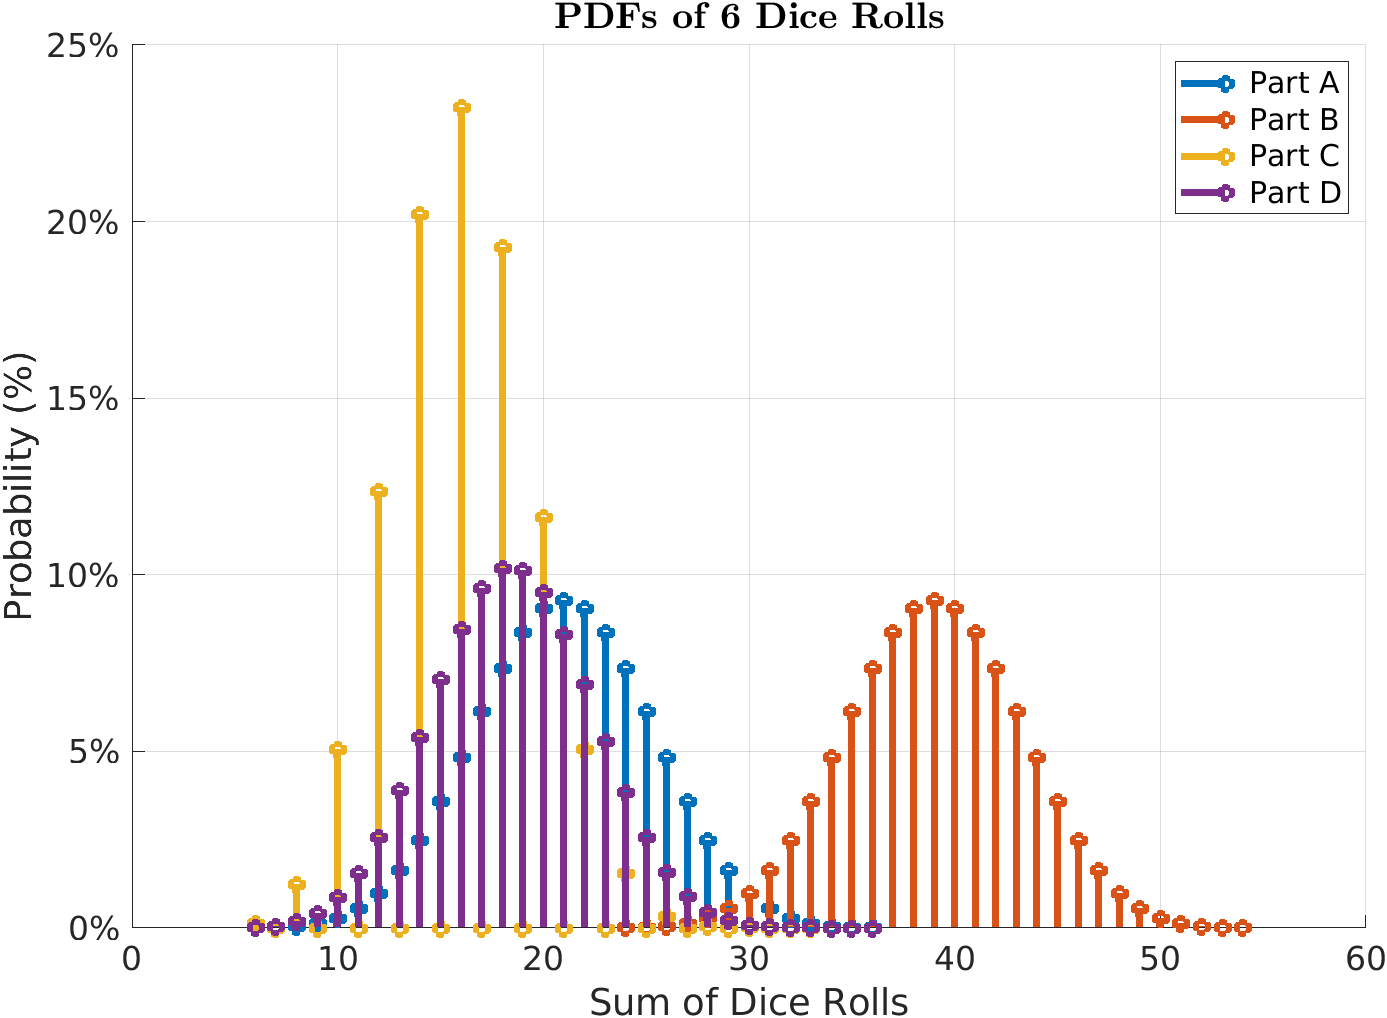
\includegraphics[width=0.65\textwidth]{p1.png}
    \caption{PDF's after Convolution.}
  \end{figure}

  % PROBLEM 2
  \item What is the joint PDF for 2 fair dice ($x_1$, $x_2$) (a 6x6 matrix 
  where each row adds to the probability index of $x_1$ and each column to 
  the probability index for $x_2$).
  \begin{enumerate}[(a)]
    \itemsep -2pt
    \item What are E\{$x_1$\}, E\{$x_1$-E\{$x_1$\}\}, E\{$x_1^2$\}, 
    E\{($x_1$-E\{$x_1$\})$^2$\} and E\{($x_1$-E\{$x_1$\})($x_2$-E\{$x_2$\})\}.
    \item Form the covariance matrix for $x_1$ and $x_2$.
    \item Find the joint PDF for $v_1=x_1$ and $v_2=x_1+x_2$.
    \item Find the mean, E\{$v_1$-E\{$v_1$\}\}, rms, and variance of $v_1$.
    \item Find the mean, E\{$v_2$-E\{$v_2$\}\}, rms, and variance of $v_2$.
    \item Find the covariance matrix of $v_1$ and $v_2$.
  \end{enumerate}
  \solution
  To create the joint PDF of two dice, the vector PDF for each dice was 
  multiplied together (each row/column sums to 1):
  \begin{equation*}
    f_{x_1x_2} = \dfrac{1}{6}.*ones(1,6)^T * \dfrac{1}{6}.*ones(1,6) = \dfrac{1}{36}.*ones(6,6)
  \end{equation*}
  For \emph{part a}:
  \begin{equation*}
    \begin{split}
      E\{x_1\} &= \bar{x}_1 = \int x_1f_{x_1}dx = \sum_{i=1}^{6}\dfrac{1}{6}i = 3.5 \\
      E\{x_1-E\{x_1\}\} &= E\{x_1-\bar{x}_1\} = \bar{x}_1 - \bar{x}_1 = 0 \\
      E\{x_1^2\} &= \int x_1^2f_{x_1}dx = \sum_{i=1}^{6}\dfrac{1}{6}i^2 = 15.17 \\
      E\{(x_1-E\{x_1\})^2\} &= \sigma_1^2 = E\{x_1^2\} - \bar{x}_1^2 = 15.17-3.5^2 = 2.92 \\
      E\{(x_1-E\{x_1\})(x_2-E\{x_2\})\} &= E\{x_1x_2\}-\bar{x}_1\bar{x}_2 = E\{x_1\}E\{x_2\}-\bar{x}_1\bar{x_2} = 0
    \end{split}
  \end{equation*}
  For \emph{part b}:
  \begin{equation*}
    \begin{split}
      \sigma_1^2 &= \sigma_2^2 \\
      P &=
      \begin{bmatrix}
        2.92 & 0 \\ 0 & 2.92
      \end{bmatrix}
    \end{split}
  \end{equation*}
  For \emph{part c} (multiplying $f_{v_1}^T*f_{v_2}$):
  \begin{equation*}
    \begin{split}
      v_1 &= 
      \begin{bmatrix} 
        1 & 2 & 3 & 4 & 5 & 6 
      \end{bmatrix}
      \\
      v_2 &= 
      \begin{bmatrix} 
        2 & 3 & 4 & 5 & 6 & 7 & 8 & 9 & 10 & 11 & 12 
      \end{bmatrix}
      \\
      f_{v_1} &=
      \begin{bmatrix}
        \dfrac{1}{6} & \dfrac{1}{6} & \dfrac{1}{6} & \dfrac{1}{6} & \dfrac{1}{6} & \dfrac{1}{6}
      \end{bmatrix}
      \\
      f_{v_2} &=
      \begin{bmatrix}
        \dfrac{1}{36} & \dfrac{1}{18} & \dfrac{1}{12} & \dfrac{1}{9} & \dfrac{5}{36} & \dfrac{1}{6} & \dfrac{5}{36} & \dfrac{1}{9} & \dfrac{1}{12} & \dfrac{1}{18} & \dfrac{1}{36}
      \end{bmatrix}
    \end{split}
  \end{equation*}
  \begin{equation*}
    f_{v_1v_2} = 
    \begin{bmatrix}
      \dfrac{1}{216} & \dfrac{1}{108} & \dfrac{1}{72} & \dfrac{1}{54} & \dfrac{5}{216} & \dfrac{1}{36} & \dfrac{5}{216} & \dfrac{1}{54} & \dfrac{1}{72} & \dfrac{1}{108} & \dfrac{1}{216}
    \end{bmatrix}
    .*ones(6,11)
  \end{equation*}
  Now each row of $f_{v_1v_2}$ sums to $f_{v_1}$ and each column sums to $f_{v_2}$. \\
  For \emph{part d}: $v_1$ has the same values as $x_1$ (\emph{part a}).\\
  For \emph{part e}:
  \begin{equation*}
    \begin{split}
      E\{v_2\} &= \bar{v}_2 = \int v_2f_{v_2}dv = 7 \\
      E\{v_2-E\{v_2\}\} &= E\{v_2-\bar{v}_2\} = \bar{v}_2 - \bar{v}_2 = 0 \\
      E\{v_2^2\} &= \int v_2^2f_{v_2}dv = 54.83 \\
      E\{(v_2-\bar{v}_2)^2\} &= \sigma_{v2}^2 = E\{v_2^2\} - E\{v_2\}^2 = 54.83 - 7^2 = 5.83
    \end{split}
  \end{equation*}
  For \emph{part f}:
  \begin{equation*}
    \begin{split}
      E\{((x_2+x_1)-(\bar{x}_2+\bar{x}_1))^2\} &= E\{x_2^2-\bar{x}_2^2+x_1^2-\bar{x}_1^2\}= \sigma_2^2 + \sigma_1^2 = \sigma_{v2}^2 = 5.83 \\
      E\{(x_1-\bar{x}_1)((x_2+x_1)-(\bar{x}_2+\bar{x}_1))\} &= P_{12} = P_{21} = E\{x_1\} - \bar{x}_1 = \sigma_1^2 = 2.92
    \end{split}
  \end{equation*}
  \begin{equation*}
    P = 
    \begin{bmatrix} 
      \sigma_1^2 & \sigma_1^2 \\ \sigma_1^2 & \sigma_1^2+\sigma_2^2
    \end{bmatrix}
    =
    \begin{bmatrix}
      2.92 & 2.92 \\ 2.92 & 5.93
    \end{bmatrix}
  \end{equation*}

  % PROBLEM 3
  \item Two random vectors $X_1$ and $X_2$ are called uncorrelated if:
  \begin{equation*}
    E\{(X_1-\bar{X}_1)(X_2-\bar{X}_2)\} = 0
  \end{equation*}
  \begin{enumerate}[(a)]
    \itemsep -2pt
    \item Show that independent random vectors are uncorrelated.
    \item Show that uncorrelated Gaussian random vectors are independent.
  \end{enumerate}
  \solution
  For independent random vectors:
  \begin{equation*}
    \begin{split}
      E\{x_1x_2\} &= E\{x_1\}E\{x_2\} = \bar{x}_1\bar{x}_2 \\
      E\{(x_1-\bar{x}_1)(x_2-\bar{x}_2)\} &= E\{x_1x_2 - x_1\bar{x}_2 - x_2\bar{x}_1 + \bar{x}_1\bar{x}_2\}
    \end{split}
  \end{equation*}
  If independent, any combinations of the random vectors together are 0, therefore:
  \begin{equation*}
      E\{(x_1-\bar{x}_1)(x_2-\bar{x}_2)\} = 0
  \end{equation*}
  For any random Gaussian vectors:
  \begin{equation*}
    \rho_{12} = \dfrac{E\{(x_1-\bar{x}_1)(x_2-\bar{x}_2)\}}{\sigma_1\sigma_2}
  \end{equation*}
  If uncorrelated, the covariance between the vectors is 0, therefore:
  \begin{equation*}
    \begin{split}
      P_{12} &= 0 \\
      \rho_{12} &= 0
    \end{split}
  \end{equation*}

  % PROBLEM 4
  \item Consider a sequence created by throwing a pair of dice and summing the 
  numbers (-2.5, -1.5, -0.5, 0.5, 1.5, 2.5) called $V_0(k)$.
  \begin{enumerate}[(a)]
    \itemsep -2pt
    \item What is the PDF?
    \item What are the mean and variance of this sequence?
    \item If we generate a new random sequence ($V_N(k+1)=(1-r)V_N(k)+rV_0(k)$) 
    ($V_N$ is serially correlated, not white). In steady-state, what are the 
    mean and variance of the new sequence?
    \item What is the covariance function: $R(k)=E\{V_N(k)V_N(k-L)\}$ (Hint: 
    $V_N(k)$ and $V_0(k)$ are uncorrelated).
    \item Are there any practical constraints on $r$?
  \end{enumerate}
  \solution
  Using the MATLAB \emph{conv} function two make the PDF for the sum 
  of two dice rolls:
  \begin{equation*}
    \begin{split}
      V_0 &=
      \begin{bmatrix}
        -5 & -4 & -3 & -2 & -1 & 0 & 1 & 2 & 3 & 4 & 5
      \end{bmatrix}
      \\ f_{V_0} &= 
      \begin{bmatrix} 
        \dfrac{1}{36} & \dfrac{1}{18} & \dfrac{1}{12} & \dfrac{1}{9} & \dfrac{5}{36} & \dfrac{1}{6} & \dfrac{5}{36} & \dfrac{1}{9} & \dfrac{1}{12} & \dfrac{1}{18} & \dfrac{1}{36}
      \end{bmatrix}
    \end{split}
  \end{equation*}
  Calculating the mean and variance of $V_0$:
  \begin{equation*}
    \begin{split}
      \mu_{V_0} &= \sum_{i=1}^{11} f_{V_0}(i)V_0(i) = 0\\
      \sigma_{V_0}^2 &= \sum_{i=1}^{11} \left(f_{V_0}(i)V_0^2(i)\right) - \mu_{V_0}^2 = 5.83
    \end{split}
  \end{equation*}
  For the system, $V_N(k+1)=(1-r)V_N(k)+rV_0(k)$, the mean of $V_N$ can 
  be assumed to be zero because it is made entirely from $V_0$, which 
  is zero mean. However, an analytical solution for the variance was 
  unable to be determined. Instead, an emperical (monte-carlo) approach 
  was used, described in the code and figure below.
  \begin{lstlisting}
  % special dice
  prob4.dice = [-2.5, -1.5, -0.5, 0.5, 1.5, 2.5];

  % initialization
  i = 1;
  prob4.VN_var = zeros(100,1);
  prob4.VN_mean = zeros(100,1);

  % r values
  for r = linspace(0,1.9,100)
      % reset
      prob4.V0 = zeros(10000,1);
      prob4.VN = zeros(10000,1);

      % monte carlo runs
      for k = 1:10000
          prob4.V0(k) = sum([prob4.dice(randi(6)), prob4.dice(randi(6))]);
          prob4.VN(k+1) = (1-r)*prob4.VN(k) + r*prob4.V0(k);
      end
      
      % get statistics
      prob4.VN_var(i) = var(prob4.VN);
      prob4.VN_mu(i) = mean(prob4.VN);
      i = i + 1;
  end
  \end{lstlisting}
  \begin{figure}[H]
    \centering
    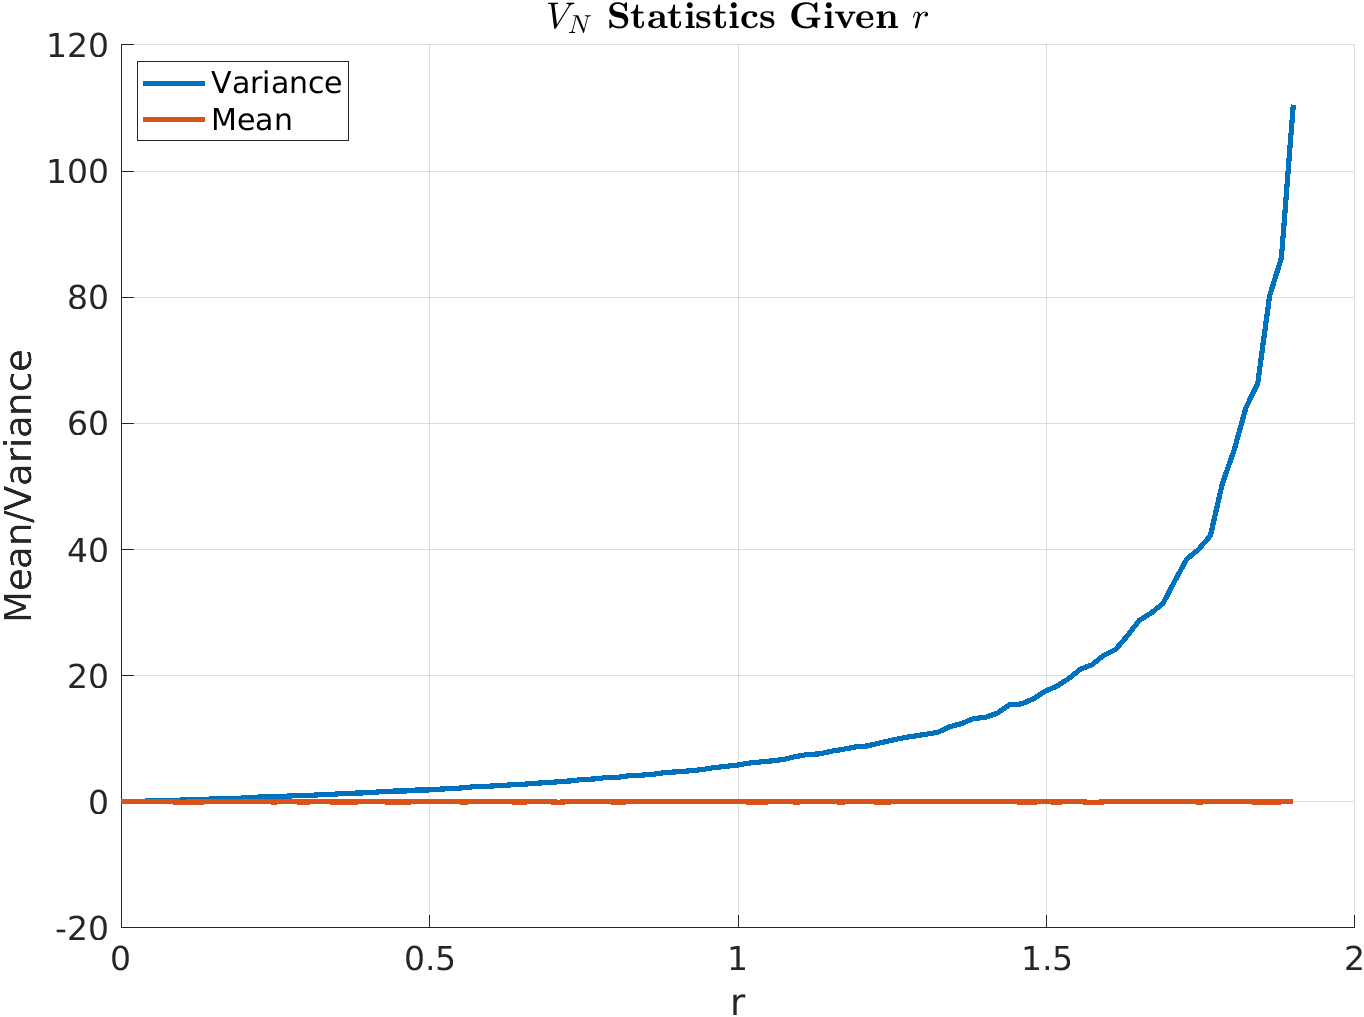
\includegraphics[width=0.65\textwidth]{p4.png}
    \caption{Mean and Variance From Monte-Carlo Simulation.}
  \end{figure}
  This proves that the mean is approximately zero and the provides insight 
  that the variance is exponentially related to $r$. \\
  The autocorrelation function (covariance) for the system is as follows:
  \begin{equation*}
    R(k) = E\{V_N(k)V_N(k+L)\}
  \end{equation*}
  Because $V_N$ is serially correlated, at can be assumed that the process 
  is stationary and the autocorrelation function can be rewritten.
  \begin{equation*}
    \begin{split}
      R(k) &= E\{V_N(k)V_N(k)\} \\
      &= E\{(V_N(k))^2\} \\
      &= E\{((1-r)V_N(k)+rV_0(k))^2\} \\
      &= E\{V_0^2(k)r^2 - 2V_0(k)V_N(k)r^2 + 2V_0(k)V_N(k)r + V_N^2(k)r^2 - 2V_N^2(k)r + V_N^2(k)\} \\
      &= E\{V_0^2(k)r^2 + V_N^2(k)r^2 - 2V_N^2r + V_N^2(k)\} \\
      &= E\{V_0^2(k)r^2 + V_N^2(k)[r^2 - 2r + 1]\}
    \end{split}
  \end{equation*}
  Analyzing this expectation, it can be determined that $r$ must remain 
  between 0 and 1, otherwise the system would have unbounded error 
  (to be completely stable, $r$ must be 0). Specifically, $r<0$ is 
  completely unstable and $r>0$ grows exponentially, quickly.

  % PROBLEM 5
  \item A random variable $x$ has a PDF given by:
  \[ f_X(x) = 
  \begin{cases}
    \mbox{$0$,           } & \mbox{} x<0 \\
    \mbox{$\dfrac{x}{2}$,} & \mbox{} 0 \leq x \leq 2 \\
    \mbox{$0$,           } & \mbox{} x>2
  \end{cases} \]
  \begin{enumerate}[(a)]
    \itemsep -2pt
    \item What is the mean of $x$?
    \item What is the variance of $x$?
  \end{enumerate}
  \solution
  For the piecewise function, $x$ only exists in the second function, therefore 
  the mean and variance of $x$ are taken only from that portion.
  \begin{equation*}
    \begin{split}
      \mu_x &= \int_{0}^{2} x\dfrac{x}{2}dx = \dfrac{1}{2}(\dfrac{1}{3}x^3)\biggr\rvert_0^2 = \dfrac{4}{3} \\
      \sigma_x^2 &= \int_{0}^{2} x^2\dfrac{x}{2}dx - \mu_x^2 = \dfrac{1}{2}(\dfrac{1}{4}x^4)\biggr\rvert_0^2 - \mu_x^2 = \dfrac{2}{9}
    \end{split}
  \end{equation*}

  % PROBLEM 6
  \item Consider a normally distributed 2D vector $x$, with a mean of 0 and 
  \begin{equation*}
    P_x = 
    \begin{bmatrix}
      2 & 1 \\ 1 & 4
    \end{bmatrix}
  \end{equation*}
  \begin{enumerate}[(a)]
    \itemsep -2pt
    \item Find the eigenvalues of $P_x$
    \item The likelihood ellipses are given by and equation of the form: 
    $x^TP_x^{-1}x=k^2$. What are the principal axes in this case.
    \item Plot the likelihood ellipses for k = 0.25, 1, 1.5.
    \item What is the probability of finding $x$ inside of each of these ellipses?
  \end{enumerate}
  \solution
  Using MATLAB's \emph{eig} function:
  \begin{equation*}
    \begin{split}
      s &= \begin{matrix} 1.5858, & 4.4142 \end{matrix} \\
      V &= \begin{bmatrix} -0.9239 & 0.3827 \\ 0.3827 & 0.9239 \end{bmatrix}
    \end{split}
  \end{equation*}
  The principal component directions and magnitude are the eigenvalues and 
  eigenvectors solved above where the principal axes are the lines spanned by 
  the eigenvectors. Below is a plot of the specified ellipses:
  \begin{figure}[H]
    \centering
    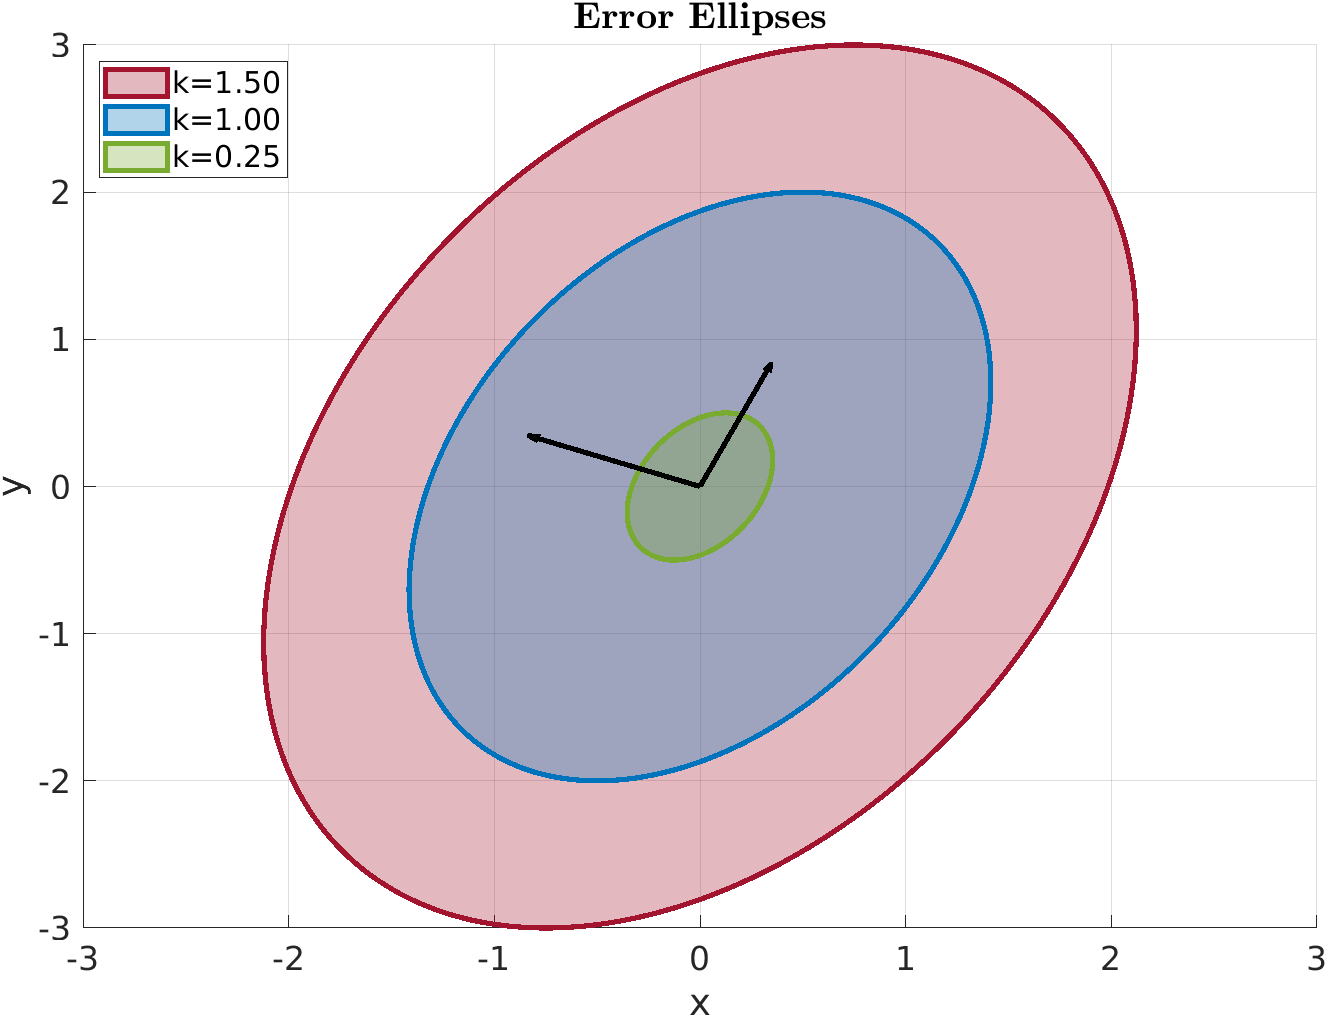
\includegraphics[width=0.65\textwidth]{p6.png}
    \caption{Specified Error Ellipses.}
  \end{figure}
  Created using the following steps:
  \begin{lstlisting}
  % covariance matrix
  prob6.P = [2, 1; 1, 4];

  % eigenvalues/vectors of covariance
  [prob6.v, prob6.s] = eig(prob6.P);

  % create the transformation matrix
  prob6.Ainv = inv(prob6.s^(-1/2) * prob6.v);

  % create a circle
  prob6.theta = 0:360;
  prob6.a = [cosd(prob6.theta); sind(prob6.theta)];

  % transform the circle into an ellipse of specifed size
  prob6.b1 = prob6.Ainv * (0.25 .* prob6.a);
  prob6.b2 = prob6.Ainv * (1.00 .* prob6.a);
  prob6.b3 = prob6.Ainv * (1.50 .* prob6.a);
  \end{lstlisting}
  To determine the likelihood of a value falling in any of the ellipses, the 
  likelihood was linearly interpolated using the $k$ values given and the table 
  provided. This results in the following percentages:
  \begin{equation*}
    \begin{split}
      \%_{k=0.25} &= 9.8350 \% \\
      \%_{k=1.00} &= 39.3400 \% \\
      \%_{k=1.50} &= 63.3333 \% \\
    \end{split}
  \end{equation*}

  % PROBLEM 7
  \item Given $x ~ N(0,\sigma_x^2)$ and $y=2x^2$:
  \begin{enumerate}[(a)]
    \itemsep -2pt
    \item Find the PDF of $y$.
    \item Draw the PDF's of $x$ and $y$ on the same plot for $\sigma_x=2.0$.
    \item How has the density function changed by this transformation?
    \item Is $y$ a normal random variable?
  \end{enumerate}
  \solution
  Given the statistics of $x$, its PDF is:
  \begin{equation*}
    f_X(x) = \dfrac{1}{\sqrt{2\pi}\sigma_x}\exp{\left(\dfrac{-1}{2}\dfrac{x^2}{\sigma_x^2}\right)}
  \end{equation*} 
  Relating $x$ to $y$:
  \begin{equation*}
    \begin{split}
      g^{-1}(y) &= x = \left(\dfrac{y}{2}\right)^{\dfrac{1}{2}} \\
      \dfrac{\partial g^{-1}(y)}{\partial y} &= \dfrac{1}{2} \left(\dfrac{y}{2}\right)^{\dfrac{-1}{2}}
    \end{split}
  \end{equation*}
  Using the relation:
  \begin{equation*}
    \begin{split}
      f_Y(y) &= f_X(g^{-1}(y)) \biggr\rVert \dfrac{\partial g^{-1}(y)}{\partial y} \biggr\rVert \\
      f_Y(y) &= \biggr\rVert \dfrac{1}{2} \left(\dfrac{y}{2}\right)^{\dfrac{-1}{2}} \biggr\rVert 
                \dfrac{1}{\sqrt{2\pi}\sigma_x}
                \exp{\left(\dfrac{-1}{2}\dfrac{\left(\left(\dfrac{y}{2}\right)^{\dfrac{1}{2}}\right)^2}{\sigma_x^2}\right)}
    \end{split}
  \end{equation*}
  Using these two PDF's to create a plot:
  \begin{figure}[H]
    \centering
    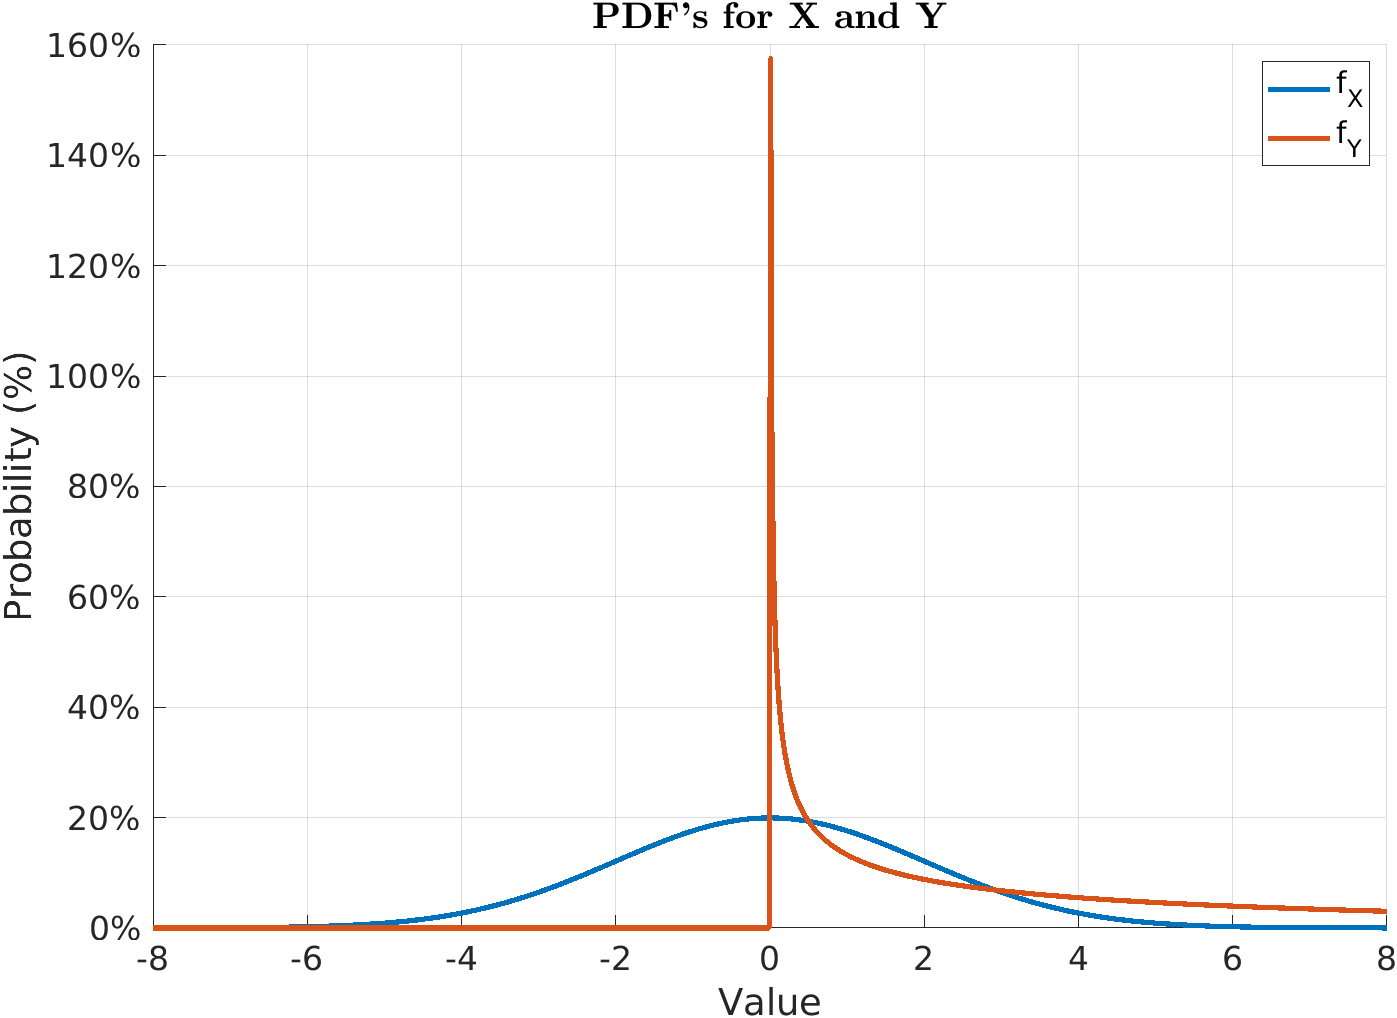
\includegraphics[width=0.65\textwidth]{p7.png}
    \caption{PDFs for x and y.}
  \end{figure}
  As shown, the PDF for $y$ is no longer zero mean or Gaussian as the sum of the 
  probability for all possible outcomes can not be equal to one. This is because a 
  nonlinear transformation is used on the PDF of a function assumed to be linear, 
  changing the characteristics of the function. The use of this squared term also 
  causes this to only be positive when rational. There is also no solution at 
  zero since the function approaches infinity as it heads towards zero.

\end{enumerate}

\end{document}